\documentclass[12pt,a4paper]{article}
\usepackage[T2A]{fontenc}
\usepackage[utf8]{inputenc}
\usepackage[russian]{babel}
\usepackage{amsmath}
\usepackage{amssymb}
\usepackage{graphicx}
\usepackage{floatrow}
\usepackage{booktabs}
\usepackage{wrapfig}
\usepackage{indentfirst}
\usepackage{lipsum}
\usepackage{subcaption}
\usepackage{float}
\usepackage{derivative}
\usepackage{fancyhdr}

\newcommand{\figref}[1]{(См. рис. \ref{#1})}
\newcommand{\secref}[1]{(См. раздел. \ref{#1})}

\newcommand{\e}[1]{\text{$\cdot10^{#1}$}}

\pagestyle{fancy}
\fancyhead{}
\fancyhead[L]{Работа 3.1.1}
\fancyhead[R]{}
\fancyfoot[C]{\thepage}

\author{\normalsize Выполнил: Голубович Тимур, группа Б01-108 \\
	\normalsize 14.09.2022}
\date{}

\usepackage{float}
\restylefloat{table}
\title{
	\large Отчет о выполнении лабораторной работы 3.1.1 \\
	\Large Магнитометр \\ 
	
}


\begin{document}
	\maketitle
	
\section*{Цель работы}
Определить горизонтальную составляющую магнитного поля Земли и установить количественное соотношение между единицами электрического тока в системах СИ и СГС.

\section*{Оборудование и приборы} 
Магнитометр;
осветитель со шкалой;
источник питания;
вольтметр;
электромагнитный переключатель;
конденсатор;
намагниченный стержень;
прибор для определения крутильных колебаний;
секундомер;
рулетка;
штангенциркуль.

\begin{figure}[H]
	\centering
	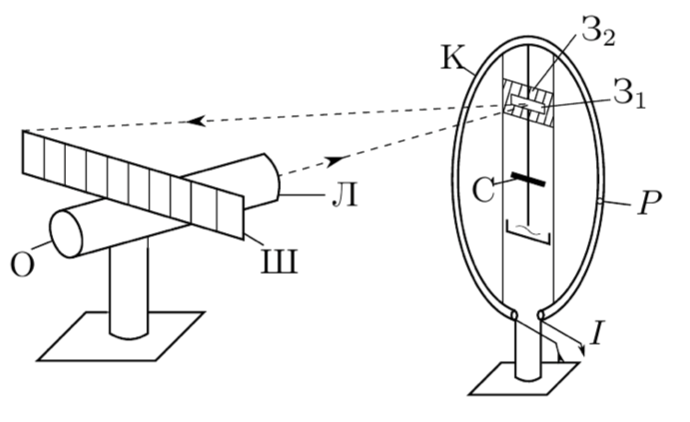
\includegraphics[width = 8 cm]{res/magnitometer.png}
	\caption{Схема магнитометра}
	\label{fig:scheme}
\end{figure}
	
\newpage
	
\section*{Теоретическое введение}

\textbf{Определение горизонтальной составляющей магнитного поля
Земли}

Поле намагниченного стержня вдали от него может быть приближённо
вычислено как поле точечного диполя:

\begin{equation}
    \textbf{B}\left(\textbf{r}\right)=\frac{\mu_0}{4\pi} \left( 3\frac{\left(\mathfrak{m}\cdot \textbf{r}\right)\textbf{r}}{r^5}-\frac{\mathfrak{m}}{r^3}\right),
    \label{eq:bio}
\end{equation}

где $\mathfrak{m}$ магнитный момент стержня, $\textbf{r}$ — радиус-вектор, проведённый из центра диполя в точку наблюдения. На оси, перпендикулярной стержню, имеем

\begin{equation}
    B_1 = \frac{\mu_0}{4\pi}\frac{\mathfrak{m}}{R^3},
    \label{eq:B1}
\end{equation}

где R - радиус кольца.
Магнитное поле в центре кольца с током по закону Био - Савара - Лапласа равно

\begin{equation}
    B_2 = \frac{\mu_0 I}{2R}N.
    \label{eq:B2}
\end{equation}

Здесь $N$ — число витков в кольце, $I$ — сила тока в единицах СИ (амперах).
Измерив тангенс угла отклонения стрелки:

\begin{equation}
    \tg \varphi_1 = \frac{x_1}{2L},
    \label{eq:phi}
\end{equation}

можно с помощью уравнений (\ref{eq:B1}), (\ref{eq:Bperp}) и (\ref{eq:phi}) рассчитать поле $B_0$, если исключить магнитный момент стержня $\mathfrak{m}$.
Связь $B_0$ и $B_\perp$($B_1$ и $B_2$):

\begin{equation}
    B_\perp = B_0 \cdot \tg \varphi.
    \label{eq:Bperp}
\end{equation}

Для исключения магнитного момента можно измерить период крутильных колебаний стержня в поле Земли. Если ось стержня отклонить в горизонтальной плоскости от
направления $B_0$ на малый угол $\alpha$, то под действием возвращающего механического момента

$$ M_\text{мех}=|\mathfrak{m}\times \textbf{B}|=\mathfrak{m} B_0 sin \alpha \approx \mathfrak{m} B_0 \alpha $$
    
Стержень с моментом инерции $J$ в соответствии с уравнением

$$\ddot{\alpha}+\mathfrak{m} B_0 \alpha = 0$$

будет совершать крутильные колебания с периодом

\begin{equation}
    T = 2\pi \sqrt{\frac{J}{\mathfrak{m} B_0}}.
    \label{eq:t}
\end{equation}

Момент инерции цилиндрического стержня относительно оси вращения

\begin{equation}
    J = m\left(\frac{l^2}{12}+\frac{r^2}{4}\right)=\frac{m l^2}{12}\left[1+3\left(\frac{r}{l}\right)^2\right],
    \label{eq:J}
\end{equation}

где $m$ - масса стержня, $l$ - длина, а $r$ - его радиус.

Таким образом, рассчитав момент инерции и измерив тангенс угла
отклонения стрелки $\phi_1$ и период малых крутильных колебаний стержня $T$, можно с помощью формул (\ref{eq:B1}), (\ref{eq:Bperp}), (\ref{eq:phi}) и (\ref{eq:t}) определить горизонтальную составляющую магнитного поля Земли:

\begin{equation}
    B_0=\frac{2\pi}{T R} \sqrt{\frac{\mu_0 J L}{2 \pi R x_1}} \;\;\; \left[\text{ед. СИ}]\right.
    \label{eq:B0}
\end{equation}

\textbf{Определение электродинамической постоянной.}

Пропуская некоторый ток через витки магнитометра, измерим тан­
генс угла отклонения стрелки ($\tg \varphi_2 = x_2/2L$) и по формулам (\ref{eq:B2}) и (\ref{eq:Bperp})
рассчитаем силу тока:

\begin{equation}
    I=\frac{2 B_0 R}{\mu_0 N} \tg \varphi_2 \;\;\; \left[\text{ед. СИ}\right].
    \label{eq:Isi}
\end{equation}

Величина $A = 2 B_0 R/\left(\mu_0 N\right)$ - постоянная прибора с поправкой на место в комнате.

Тот же ток можно измерить абсолютным образом по прошедшему в единицу времени заряду, что соответствует определению эталона тока в гауссовой системе (СГС). Если разрядить конденсатор известной
ёмкости $C$, заряженный до напряжения $U$, через витки, то через них
протечёт заряд $q=CU$(рис. $\ref{fig:coil}$). Если $\nu$ раз в секунду последовательно
заряжать конденсатор от источника и разряжать через витки, то через
них за секунду протечёт заряд $CU\nu$. Средний ток, прошедший через
витки, равен при этом

\begin{equation}
    I=CU\nu \;\;\; \left[\text{абс. ед}\right].
    \label{eq:Isgs}
\end{equation}

Итак, для вычисления абсолютного значения тока по (\ref{eq:Isgs}) необходимо
измерить напряжение $U$ на конденсаторе известной ёмкости $C$. Напряжение необходимо выразить $\textit{в единицах СГС}$ (измерительные приборы,
как правило, проградуированы в единицах СИ: $1 \text{В} \approx\frac{1}{300}$ ед. СГС).
Ёмкость конденсатора $C$ [см] должна быть выражена в $\textit{сантиметрах}$
$(1 \text{Ф} \approx 9 \cdot 10^{11} \text{см})$.

По отношению численных значений одного и того же тока, выражен­
ных в единицах СИ и СГС (гауссовой) по формулам (\ref{eq:Isi}) и (\ref{eq:Isgs}) соответственно, можно определить значение электродинамической постоянной:

\begin{equation}
    c\left[\frac{\text{м}}{\text{с}}\right]=\frac{1}{10}\frac{I_{\left[\text{СГС}\right]}}{I_{\left[\text{СИ}\right]}}=\frac{1}{10}CU\nu\frac{\mu_0 N}{2B_0 R \tg \varphi_2}.
    \label{eq:c}
\end{equation}

\section*{Экспериментальная установка}

Магнитометр (рис. \ref{fig:scheme}) состоит из нескольких последовательно соединённых круговых витков $K$, расположенных вертикально. В центре кольца $K$ радиусом на тонкой неупругой вертикальной нити подвешена короткая магнитная стрелка $C$. Жёстко связанная со стрелкой крыльчатка погружена в масло и служит для демпфирования колебаний.

\begin{figure}[H]
	\centering
	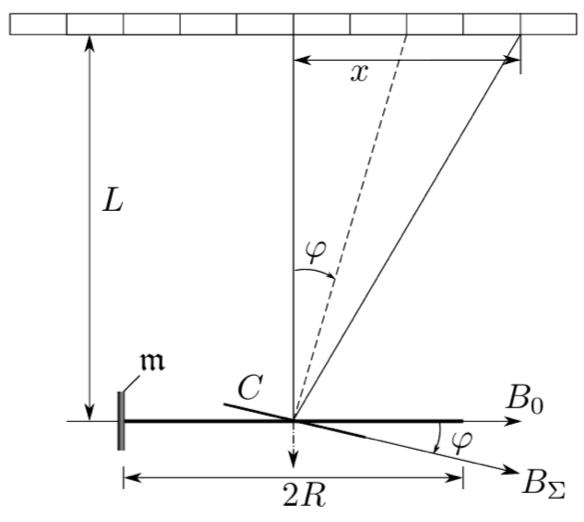
\includegraphics[width = 8 cm]{res/angle_facility.png}
	\caption{Схема измерения угла отклонения магнитной стрелки}
	\label{fig:angle}
\end{figure}

\begin{figure}[H]
	\centering
	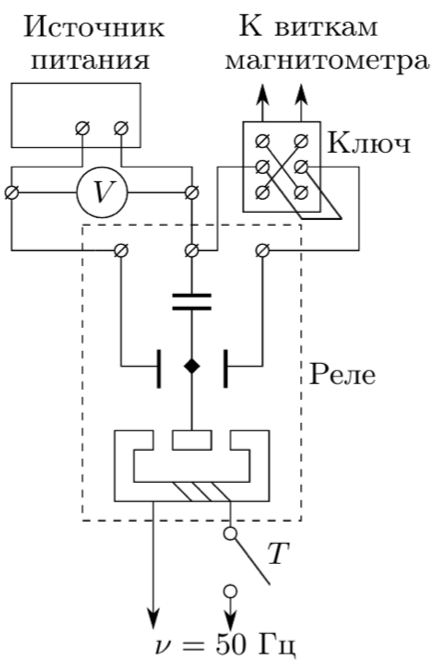
\includegraphics[width = 8 cm]{res/coil.png}
	\caption{Схема питания катушки магнитометра}
	\label{fig:coil}
\end{figure}

Прибор настраивают с помощью световых зайчиков, отражённых от
двух зеркал: $\text{З}_1$, прикреплённого к стрелке (подвижный зайчик), и $\text{З}_2$,
расположенного в плоскости кольца $K$ и жёстко связанного с ним (неподвижный зайчик). Оба зеркала освещаются одним и тем же осветителем $O$. Вращением кольца вокруг вертикальной оси можно совместить
оба зайчика. При этом плоскость витков совпадает с плоскостью магнитного меридиана.

\newpage

\section*{Ход работы}

\subsection*{Измерение горизонтальной составляющей магнитного поля Земли}

Запишем все параметры установки, входящие в формулу (\ref{eq:B0}), в таблицу \ref{tab:exp1}. В отверстие $P$ на горизонтальном диаметре кольца вставим
намагниченный стержень и измерим смещение подвижного зайчика. Результат занесём туда же. После поменяем ориентацию стержня в гнезде и измерим отклонение зайчика в другую сторону. Оно составляет $x^\prime_1=8,1 \; \text{см}$. Таким образом разница $|x_1-x^\prime_1|=0,4 \; \text{см}$, что составляет $\varepsilon=4,7\; \%$.

Найдём количество колебаний, необходимое для вычисления периода одного колебания с погрешностью с погрешностью $\varepsilon_T<1\%$. Основная ошибка измерения - это человеческий фактор, который $\sigma_T \approx 1 \; \text{с}$. Период одного колебания $T \approx 7 \; \text{с}$. Тогда можно составить уравнение:
    $$\frac{\sigma_T}{n \cdot T} = \varepsilon_T \Rightarrow n = \frac{\sigma_T}{T\cdot \varepsilon_T} \approx 15 \; \text{колебаний.}$$
Округлим для удобства полученное значение до 20.

\begin{table}[H]
	\caption{Таблица для измерения $B_0$}
	\begin{tabular}{cccccccc}
\toprule
                 &$m$, г&$d$, мм&$l$, мм&$T_{20}$, с&$R$, см&$L$, см&$x_1$, см\\
\midrule
                 &5,987 &0,5    &3,99   &136,25   &20     &112    &8,5      \\
$\sigma$         &0,001 &0,01   &0,01   &1,0      &-      &1,0    &0,1      \\
$\varepsilon$, \%&0,017 &2      &0,3    &0,7      &-      &0,9    &1,2      \\
\bottomrule
\end{tabular}

	\label{tab:exp1}
\end{table}

По формуле (\ref{eq:B0}) рассчитаем горизонтальную составляющую поля Земли: $B_0 = 15,1 \; \text{мкТл}$.

Для оценки погрешности сразу пренебрежем погрешностями $\sigma_m$ и $\sigma_l$ ввиду их малости по сравнению с остальными. Погрешность поля $B_0$ рассчитаем по следующей формуле:
$$\sigma_{B_0}=\sqrt{\left(\frac{\partial B_0}{\partial J}\frac{\partial J}{\partial d}\sigma_d \right)^2+\left(\frac{\partial B_0}{\partial T}\sigma_T \right)^2+\left(\frac{\partial B_0}{\partial L}\sigma_L \right)^2+\left(\frac{\partial B_0}{\partial x_1}\sigma_{x_1} \right)^2}.$$

Таким образом $B_0=\left(15,1\pm1,5\right) \; \text{мкТл}, \; \varepsilon_{B_0}=10\%$.

\newpage


\subsection*{Измерение электродинамической постоянной}

Проведём измерения в соответствии с инструкцией. Отклонение зайчика в одну сторону $x^\prime_2=10,9 \; \text{см}$, отклонение в другую $x^{\prime\prime}_2=11,4 \; \text{см}$. Разница $|x^\prime_2-x^{\prime\prime}_2|=0,5 \; \text{см}$, что составляет $\varepsilon=4,3\; \%$. Эта разница опять таки $<5\%$, поэтому можно продолжать измерения. Результаты занесём в таблицу \ref{tab:exp2}.

\begin{table}[H]
	\caption{Таблица для измерения $c$}
	\begin{tabular}{cccccccc}
\toprule
                 &$С\cdot10^5$,\;см&$U$,\;В&$\nu$,\;$\text{c}^{-1}$&$N$,\;витков&$B_0$,\;мкТл&$R$,\;см&$x_2$,\;см\\
\midrule
                 &9              &98   &50      &44        &15,1      &20    &11,1    \\
$\sigma$         &0,18           &1,0  &-       &-         &0,15      &-     &0,10    \\
$\varepsilon$, \%&2              &1,0  &-       &-         &10        &-     &1,2     \\
\bottomrule
\end{tabular}

	\label{tab:exp2}
\end{table}

Рассчитаем токи в СИ и СГС, предварительно переведя В в ед. СГС:

$$I_{\left[\text{СГС}\right]}=1,47\cdot10^7\;\text{[ед. СГС]}$$
$$I_{\left[\text{СИ}\right]}=5,43\cdot10^{-3}\;\text{[ед. СИ]}$$

Погрешность величины $c$ можно рассчитать по формуле погрешностей для косвенных измерений:

$$\sigma_c=\sqrt{ \sum\limits_{i=1}^n \left(\frac{\partial c}{\partial x_i}\sigma_{x_i} \right)^2},$$

где $x_i$ - величина, входящая в формулу для $c$ и обладающая некоторой погрешностью.

Таким образом электродинамическая постоянная:
$$c=(2,71\pm0,3)\cdot 10^8 \; \frac{\text{м}}{\text{с}}, \; \varepsilon_c=12\%.$$
Истинную погрешность можно найти по такой формуле:
$$\sigma_c=\frac{c_\text{истин}-c}{c_\text{истин}}=10\%.$$

\newpage

\section*{Вывод}

В ходе работы были получены следующие величины для горизонтальной составляющей магнитного поля Земли и электродинамической постоянной:

$$B_0=\left(15,1\pm1,5\right) \; \text{мкТл}, \; \varepsilon_{B_0}=10\%$$
$$c=(2,71\pm0,3)\cdot 10^8 \; \frac{\text{м}}{\text{с}}, \; \varepsilon_c=12\%.$$

Согласно приведенным в конце источникам, реальная величина магнитного поля Земли колеблется от 25 до 65 мкТл.
Полученная в ходе работы величина несколько ниже приведенных. Возможно, расхождения возникли из-за того, что измерения проводились в бетонном здании. Что касается электродинамической постоянной, то её значение с учетом погрешности совпадает с табличным $3\cdot10^8\;\frac{\text{м}}{\text{с}}$. Истинная погрешность $\sigma_c=10\%$.


\begin{thebibliography}{4}
	\bibitem{Siv} Сивухин Д. В. \emph{Общий курс физики. Том 3 Электричество и магнетизм}, 2004
	\bibitem{kirich} Кириченко Н.А. \emph{Электричество и магнетизм.}, 2011
	\bibitem{max} \emph{Лабораторный практикум по общей физике. В 3 томах. Том 2. Электричество и магнетизм: учебное пособие} под ред. А. В. Максимычева, М. Г. Никулина
	\bibitem{wiki} \emph{https://ru.wikipedia.org/wiki/Магнитное\_поле\_Земли}
\end{thebibliography}
\end{document}
